\documentclass[usenames,dvipsnames]{beamer}[12pt]
\usetheme{boxes}
\usecolortheme{seahorse}

\setbeamerfont{page number in head/foot}{size=\footnotesize}

\setbeamertemplate{navigation symbols}{}
\setbeamertemplate{items}[triangle]
\setbeamertemplate{footline}[frame number]

\usepackage{graphicx}
\usepackage{listings}
\usepackage{color}
\usepackage{tikz}
\usepackage{tkz-graph}
\usepackage{csvsimple}
\usepackage{filecontents}
\usepackage{pgfplots}
\usetikzlibrary{hobby}   
\usetikzlibrary{fit}
\usepackage{xcolor}

\usepackage{bera}% optional: just to have a nice mono-spaced font

\colorlet{punct}{red!60!black}
\definecolor{background}{HTML}{EEEEEE}
\definecolor{delim}{RGB}{20,105,176}
\colorlet{numb}{magenta!60!black}

\lstdefinelanguage{json}{
	basicstyle=\normalfont\ttfamily,
	numbers=left,
	numberstyle=\scriptsize,
	stepnumber=1,
	numbersep=8pt,
	showstringspaces=false,
	breaklines=true,
	frame=lines,
	backgroundcolor=\color{background},
	literate=
	*{0}{{{\color{numb}0}}}{1}
	{1}{{{\color{numb}1}}}{1}
	{2}{{{\color{numb}2}}}{1}
	{3}{{{\color{numb}3}}}{1}
	{4}{{{\color{numb}4}}}{1}
	{5}{{{\color{numb}5}}}{1}
	{6}{{{\color{numb}6}}}{1}
	{7}{{{\color{numb}7}}}{1}
	{8}{{{\color{numb}8}}}{1}
	{9}{{{\color{numb}9}}}{1}
	{:}{{{\color{punct}{:}}}}{1}
	{,}{{{\color{punct}{,}}}}{1}
	{\{}{{{\color{delim}{\{}}}}{1}
	{\}}{{{\color{delim}{\}}}}}{1}
	{[}{{{\color{delim}{[}}}}{1}
	{]}{{{\color{delim}{]}}}}{1},
	string=[s]{"}{"}
}

\newcommand\blfootnote[1]{%
	\begingroup
	\renewcommand\thefootnote{}\footnote{#1}%
	\addtocounter{footnote}{-1}%
	\endgroup
}

\newcommand\irregularcircle[2]{% radius, irregularity
	\pgfextra {\pgfmathsetmacro\len{(#1)+rand*(#2)}}
	+(0:\len pt)
	\foreach \a in {10,20,...,350}{
		\pgfextra {\pgfmathsetmacro\len{(#1)+rand*(#2)}}
		-- +(\a:\len pt)
	} -- cycle
}

\begin{document}
	
	\title{Presentation 5}
	\author{Fynn Lohren, Carsten Schubert, Leon Suchy}
	\date{\today}
	\frame{\titlepage}
	
	\begin{frame}
		\frametitle{Profiling \& Optimization}
		
		\begin{itemize}
			\item Measured times with Perf
			\item Lots of tiny optimizations
			\item Most time spent with reductions
			
			\pause
			
			\item Optimize 2-fold
			\item Build meta data late
			\item Apply initial reductions
		\end{itemize}
	\end{frame}

	\begin{frame}
		\frametitle{Old 2-fold}
		
		\begin{center}
			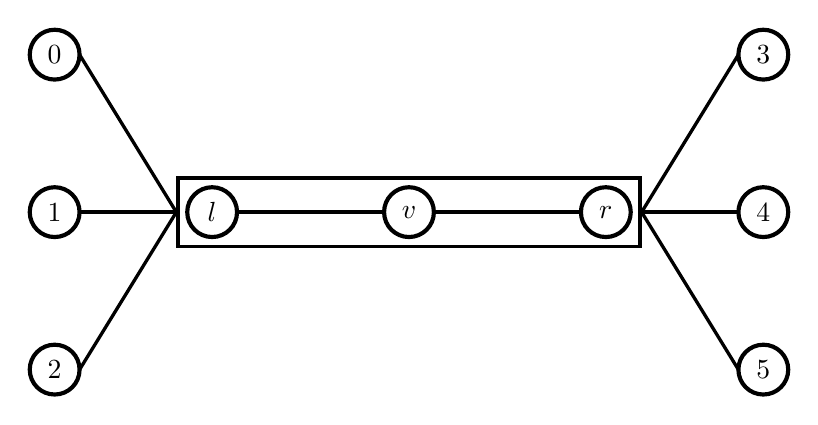
\begin{tikzpicture}
			%\draw[help lines] (0,0) grid (6,1);
			
			\SetVertexNormal[
			Shape 		= circle,
			LineWidth 	= 1.5pt]
			\SetUpEdge[
			lw 		= 1.5pt,
			color 	= black]
			
			\Vertex[x=0,y=4,L=$0$]{4}
			\Vertex[x=0,y=2,L=$1$]{5}	
			\Vertex[x=0,y=0,L=$2$]{6}
			
			\Vertex[x=9,y=4,L=$3$]{7}
			\Vertex[x=9,y=2,L=$4$]{8}	
			\Vertex[x=9,y=0,L=$5$]{9}
			
			\Vertex[x=2,y=2,L=$l$]{1}
			\Vertex[x=4.5,y=2,L=$v$]{2}
			\Vertex[x=7,y=2,L=$r$]{3}
			
			\begin{scope}
			\node[fit = (1)(2)(3),draw=black, very thick] (group-inner) {};
			\end{scope}
			
			\path[every node/.style={font=\sffamily\small},very thick]
			(4.east) edge (group-inner.west)
			(5.east) edge (group-inner.west)
			(6.east) edge (group-inner.west)
			(group-inner.east) edge (7.west)
			(group-inner.east) edge (8.west)
			(group-inner.east) edge (9.west);
			
			\Edges(1,2,3);
			
			\end{tikzpicture}
		\end{center}
		
	\end{frame}

	\begin{frame}
		\frametitle{Better 2-fold}
		
		\begin{center}
			Use middle vertex to represent the group
			
			\vspace{2mm}
			
			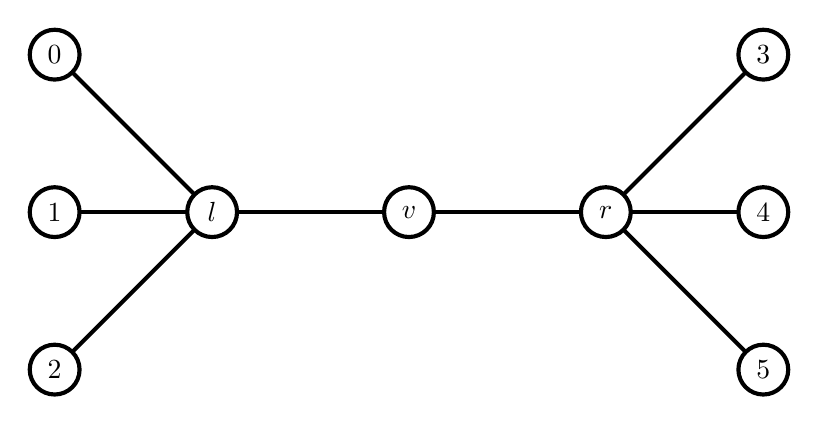
\begin{tikzpicture}
			%\draw[help lines] (0,0) grid (9,4);
			
				\SetVertexNormal[
				Shape 		= circle,
				LineWidth 	= 1.5pt]
				\SetUpEdge[
				lw 		= 1.5pt,
				color 	= black]
			
				\Vertex[x=0,y=4,L=$0$]{0}
				\Vertex[x=0,y=2,L=$1$]{1}	
				\Vertex[x=0,y=0,L=$2$]{2}
				
				\Vertex[x=9,y=4,L=$3$]{3}
				\Vertex[x=9,y=2,L=$4$]{4}	
				\Vertex[x=9,y=0,L=$5$]{5}
				
				\Vertex[x=2,y=2,L=$l$]{6}
				\Vertex[x=4.5,y=2,L=$v$]{7}
				\Vertex[x=7,y=2,L=$r$]{8}
				
				\Edges(0,6)
				\Edges(1,6)
				\Edges(2,6)
			
				\Edges(3,8)
				\Edges(4,8)
				\Edges(5,8)
				
				\Edges(6,7)
				\Edges(7,8)
			
			\end{tikzpicture}
		\end{center}
	
	\end{frame}

	\begin{frame}
		\frametitle{Better 2-fold}
		
		\begin{center}
			Use middle vertex to represent the group
			
			\vspace{2mm}
			
			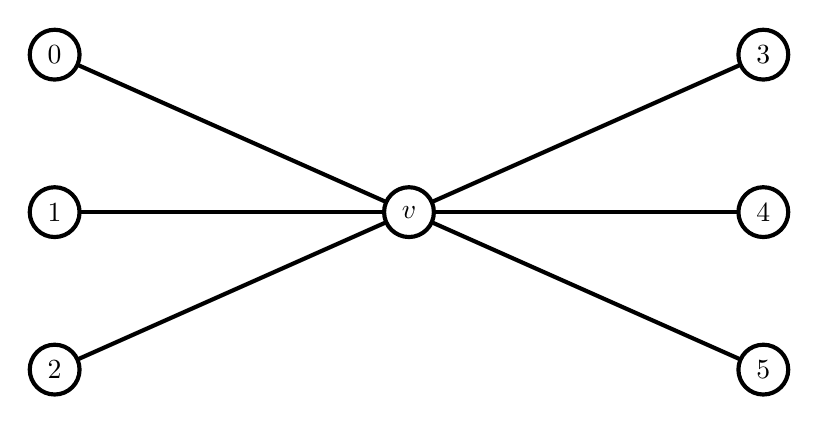
\begin{tikzpicture}
			%\draw[help lines] (0,0) grid (9,4);
			
			\SetVertexNormal[
			Shape 		= circle,
			LineWidth 	= 1.5pt]
			\SetUpEdge[
			lw 		= 1.5pt,
			color 	= black]
			
			\Vertex[x=0,y=4,L=$0$]{0}
			\Vertex[x=0,y=2,L=$1$]{1}	
			\Vertex[x=0,y=0,L=$2$]{2}
			
			\Vertex[x=9,y=4,L=$3$]{3}
			\Vertex[x=9,y=2,L=$4$]{4}	
			\Vertex[x=9,y=0,L=$5$]{5}
			
			\Vertex[x=4.5,y=2,L=$v$]{7}
			
			\Edges(0,7)
			\Edges(1,7)
			\Edges(2,7)
			
			\Edges(3,7)
			\Edges(4,7)
			\Edges(5,7)
			
			\end{tikzpicture}
		\end{center}
		
	\end{frame}

	\begin{frame}
		\frametitle{Config Parameters}
		
		\begin{itemize}
			\item Maximum degree
			\item Frequency
			\item Lower bound toggles
			\item Groups
		\end{itemize}
	\end{frame}
	
	\begin{frame}[fragile]
		\frametitle{Data Reduction Groups}
		
		\begin{itemize}
			\item Always exhaustive is inefficient
			\item Once: Apply reductions non-exhaustively
			\item Exhaustive \\
			$\rightarrow$ Frequency: Every k recursion layers
		\end{itemize}
	
		\vspace{4mm}
	
		\begin{lstlisting}[language=json,firstnumber=1]
{
  "name": "once", "priority": 6, "frequency": 1,
  "data-reductions": [
    { "name": "degree > k", "priority": 5 }
  ]
}
		\end{lstlisting}
		
	\end{frame}

	\begin{frame}
		\frametitle{Overview}
		\begin{itemize}
			\item 14 Data reductions
			\item 3 Lower bounds
			\item Components
			\item Mirror Branching
			\item Kernelization
		\end{itemize}
	\end{frame}

	\begin{frame}
		\frametitle{Overview - Data Reductions}
		
		\begin{itemize}
			\item Degree 0, 1, 2, 3, 4 and >k
			\item 2: Fold, Triangle
			\item 3: Independent Set, Neighbor Clique Partition
			\item 4: Path, Crossbow, Trebuchet
			\item Dominate
			\item Unconfined
			\item Crown
			\item LP
			\item Neighbor Clique Partition
		\end{itemize}
	\end{frame}

	\begin{frame}
		\frametitle{Overview - Lower Bounds}
		
		\begin{itemize}
			\item Clique Cover
			\item Cycle Cover
			\item LP
		\end{itemize}
	\end{frame}

	\begin{frame}
		\frametitle{Retrospective}
		
		Not every theoretical concept was useful in practice \\
		\pause
		\vspace{8mm}
		Algorithmic efficiency vs. technical efficiency \\
		\pause
		\vspace{8mm}
		Organization, communication and clear goals are important\\
	\end{frame}
\end{document}